%%%%%%%%%%%%%%%%%%%%%%%%%%%%%%%%%%%%%%%%%%%%%%%%%%%%%%%%%%%%%%%%%%%%%%
% Lớp 9 | Chương VI. Hàm số y = ax² (a ≠ 0). Phương trình bậc hai một ẩn | Hàm số y = ax² (a ≠ 0)
% Dạng 9D6?18-3: Tương giao giữa parabol và đường thẳng
%%%%%%%%%%%%%%%%%%%%%%%%%%%%%%%%%%%%%%%%%%%%%%%%%%%%%%%%%%%%%%%%%%%%%%


% nguồn: 2026-11-18_chuan_hoa_45_cau_ts10_vao_lop9 (nhập 18/11/2026)
\begin{bt}%[9D6H18-3]%[ma:f6439493]
% nguon: Tuyển tập đề thi Tuyển sinh 10 TP.HCM
Cho parabol $(P): y = -x^2$ và đường thẳng $(d): y = -3x + 2$.
\textbf{a)} Vẽ đồ thị $(P)$ trên hệ trục tọa độ. \par
\textbf{b)} Tìm tọa độ giao điểm của $(P)$ và $(d)$ bằng phép tính.
\loigiai{
\textbf{a)} Vẽ đồ thị $(P): y = -x^2$ \hfill \textit{(1,0 điểm)} \par
Bảng giá trị:
\begin{center}
\begin{tabular}{|c|c|c|c|c|c|}
\hline
$x$ & $-2$ & $-1$ & $0$ & $1$ & $2$ \\
\hline
$y = -x^2$ & $-4$ & $-1$ & $0$ & $-1$ & $-4$ \\
\hline
\end{tabular}
\end{center}
Đồ thị hàm số $(P)$ là một đường parabol đi qua gốc tọa độ $O$, nhận trục $Oy$ làm trục đối xứng và nằm phía dưới trục hoành.
\begin{center}
\begin{tikzpicture}[>=stealth, scale=1]
\draw[->] (-3.5,0) -- (3.5,0) node[above] {$x$};
\draw[->] (0,-5.5) -- (0,1) node[right] {$y$};
\fill (0,0) circle (1.5pt) node[above right] {$O$};
\draw[domain=-2.2:2.2, smooth, thick] plot (\x, {-\x*\x});
\draw[dashed] (-2,0) node[above]{$-2$} |- (0,-4) node[below left]{$-4$} -| (2,0) node[above]{$2$};
\draw[dashed] (-1,0) node[above]{$-1$} |- (0,-1) node[below left]{$-1$} -| (1,0) node[above]{$1$};
\fill (-2,-4) circle (1.5pt); \fill (2,-4) circle (1.5pt);
\fill (-1,-1) circle (1.5pt); \fill (1,-1) circle (1.5pt);
\node[right] at (2.2, -4.8) {$(P)$};
\end{tikzpicture}
\end{center}
\textbf{b)} Tìm tọa độ giao điểm của $(P)$ và $(d)$ \hfill \textit{(0,5 điểm)} \par
Phương trình hoành độ giao điểm của $(P)$ và $(d)$ là:
$$ -x^2 = -3x + 2 $$
$$ \Leftrightarrow x^2 - 3x + 2 = 0 $$
Vì $a + b + c = 1 + (-3) + 2 = 0$ nên phương trình có hai nghiệm:
$$ x_1 = 1; \quad x_2 = 2 $$
Với $x = 1 \Rightarrow y = -(1)^2 = -1$. Ta được giao điểm thứ nhất là $(1; -1)$. \par
Với $x = 2 \Rightarrow y = -(2)^2 = -4$. Ta được giao điểm thứ hai là $(2; -4)$. \par
Vậy tọa độ giao điểm của $(P)$ và $(d)$ là $(1; -1)$ và $(2; -4)$.
}
\end{bt}

% nguồn: 2026-11-18_chuan_hoa_45_cau_ts10_vao_lop9 (nhập 18/11/2026)
\begin{bt}%[9D6H18-3]%[ma:c8ebd171]
% nguon: Tuyển tập đề thi Tuyển sinh 10 TP.HCM
Cho parabol $(P): y = -x^2$ và đường thẳng $(d): y = 3x - 4$.
\textbf{a)} Vẽ đồ thị $(P)$ trên hệ trục tọa độ. \par
\textbf{b)} Tìm tọa độ giao điểm của $(P)$ và $(d)$ bằng phép tính.
\loigiai{
\textbf{a)} Vẽ đồ thị $(P): y = -x^2$ \hfill \textit{(1,0 điểm)} \par
Bảng giá trị:
\begin{center}
\begin{tabular}{|c|c|c|c|c|c|}
\hline
$x$ & $-2$ & $-1$ & $0$ & $1$ & $2$ \\
\hline
$y = -x^2$ & $-4$ & $-1$ & $0$ & $-1$ & $-4$ \\
\hline
\end{tabular}
\end{center}
Đồ thị hàm số $(P)$ là một đường parabol đi qua gốc tọa độ $O$, nhận trục $Oy$ làm trục đối xứng và nằm phía dưới trục hoành.
\begin{center}
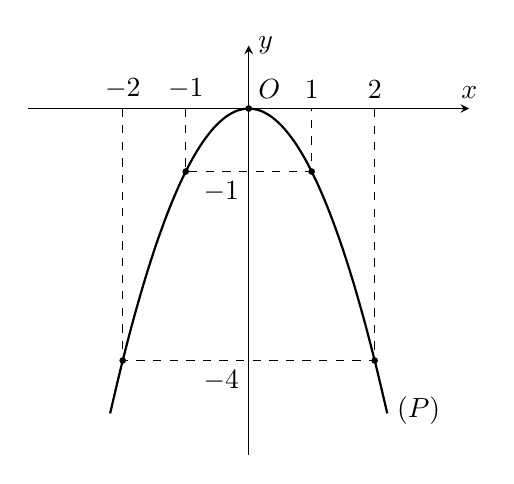
\begin{tikzpicture}[>=stealth, scale=0.8]
\draw[->] (-3.5,0) -- (3.5,0) node[above] {$x$};
\draw[->] (0,-5.5) -- (0,1) node[right] {$y$};
\fill (0,0) circle (1.5pt) node[above right] {$O$};
\draw[domain=-2.2:2.2, smooth, thick] plot (\x, {-\x*\x});
\draw[dashed] (-2,0) node[above]{$-2$} |- (0,-4) node[below left]{$-4$} -| (2,0) node[above]{$2$};
\draw[dashed] (-1,0) node[above]{$-1$} |- (0,-1) node[below left]{$-1$} -| (1,0) node[above]{$1$};
\fill (-2,-4) circle (1.5pt); \fill (2,-4) circle (1.5pt);
\fill (-1,-1) circle (1.5pt); \fill (1,-1) circle (1.5pt);
\node[right] at (2.2, -4.8) {$(P)$};
\end{tikzpicture}
\end{center}
\textbf{b)} Tìm tọa độ giao điểm của $(P)$ và $(d)$ \hfill \textit{(0,5 điểm)} \par
Phương trình hoành độ giao điểm của $(P)$ và $(d)$ là:
$$ -x^2 = 3x - 4 $$
$$ \Leftrightarrow x^2 + 3x - 4 = 0 $$
Vì $a + b + c = 1 + 3 + (-4) = 0$ nên phương trình có hai nghiệm:
$$ x_1 = 1; \quad x_2 = -4 $$
Với $x = 1 \Rightarrow y = -(1)^2 = -1$. Ta được giao điểm thứ nhất là $(1; -1)$. \par
Với $x = -4 \Rightarrow y = -(-4)^2 = -16$. Ta được giao điểm thứ hai là $(-4; -16)$. \par
Vậy tọa độ giao điểm của $(P)$ và $(d)$ là $(1; -1)$ và $(-4; -16)$.
}
\end{bt}

% nguồn: 2026-11-18_chuan_hoa_45_cau_ts10_vao_lop9 (nhập 18/11/2026)
\begin{bt}%[9D6H18-3]%[ma:a40b5424]
% nguon: Tuyển tập đề thi Tuyển sinh 10 TP.HCM
Cho parabol $(P): y = -\frac{1}{4}x^2$ và đường thẳng $(d): y = \frac{1}{2}x - 2$.
\textbf{a)} Vẽ đồ thị $(P)$ trên hệ trục tọa độ. \par
\textbf{b)} Bằng phép tính, tìm tọa độ giao điểm của $(P)$ và $(d)$.
\loigiai{
\textbf{a)} Vẽ đồ thị $(P): y = -\frac{1}{4}x^2$ \hfill \textit{(1,0 điểm)} \par
Bảng giá trị:
\begin{center}
\begin{tabular}{|c|c|c|c|c|c|}
\hline
$x$ & $-4$ & $-2$ & $0$ & $2$ & $4$ \\
\hline
$y = -\frac{1}{4}x^2$ & $-4$ & $-1$ & $0$ & $-1$ & $-4$ \\
\hline
\end{tabular}
\end{center}
Đồ thị hàm số $(P)$ là một đường parabol đi qua gốc tọa độ $O$, nhận trục $Oy$ làm trục đối xứng và nằm phía dưới trục hoành.
\begin{center}
\begin{tikzpicture}[>=stealth, scale=0.8]
\draw[->] (-5.5,0) -- (5.5,0) node[above] {$x$};
\draw[->] (0,-5.5) -- (0,1) node[right] {$y$};
\fill (0,0) circle (1.5pt) node[above right] {$O$};
\draw[domain=-4.5:4.5, smooth, thick] plot (\x, {-0.25*\x*\x});
\draw[dashed] (-4,0) node[above]{$-4$} |- (0,-4) node[below left]{$-4$} -| (4,0) node[above]{$4$};
\draw[dashed] (-2,0) node[above]{$-2$} |- (0,-1) node[below left]{$-1$} -| (2,0) node[above]{$2$};
\fill (-4,-4) circle (1.5pt); \fill (4,-4) circle (1.5pt);
\fill (-2,-1) circle (1.5pt); \fill (2,-1) circle (1.5pt);
\node[right] at (4.5, -5) {$(P)$};
\end{tikzpicture}
\end{center}
\textbf{b)} Tìm tọa độ giao điểm của $(P)$ và $(d)$ \hfill \textit{(0,5 điểm)} \par
Phương trình hoành độ giao điểm của $(P)$ và $(d)$ là:
$$ -\frac{1}{4}x^2 = \frac{1}{2}x - 2 $$
$$ \Leftrightarrow x^2 + 2x - 8 = 0 $$
$$ \Leftrightarrow (x - 2)(x + 4) = 0 $$
$$ \Leftrightarrow \heva{&x = 2 \\ &x = -4} $$
Với $x = 2 \Rightarrow y = -\frac{1}{4}(2)^2 = -1$. Ta được giao điểm thứ nhất là $(2; -1)$. \par
Với $x = -4 \Rightarrow y = -\frac{1}{4}(-4)^2 = -4$. Ta được giao điểm thứ hai là $(-4; -4)$. \par
Vậy tọa độ giao điểm của $(P)$ và $(d)$ là $(2; -1)$ và $(-4; -4)$.
}
\end{bt}

% nguồn: 2026-11-18_chuan_hoa_45_cau_ts10_vao_lop9 (nhập 18/11/2026)
\begin{bt}%[9D6H18-3]%[ma:887c2273]
% nguon: Tuyển tập đề thi Tuyển sinh 10 TP.HCM
Cho parabol $(P): y = \frac{1}{2}x^2$ và đường thẳng $(d): y = -x + 4$.
\textbf{a)} Vẽ đồ thị $(P)$ trên hệ trục tọa độ. \par
\textbf{b)} Tìm tọa độ giao điểm của $(P)$ và $(d)$ bằng phép tính.
\loigiai{
\textbf{a)} Vẽ đồ thị $(P): y = \frac{1}{2}x^2$ \hfill \textit{(1,0 điểm)} \par
Bảng giá trị:
\begin{center}
\begin{tabular}{|c|c|c|c|c|c|}
\hline
$x$ & $-4$ & $-2$ & $0$ & $2$ & $4$ \\
\hline
$y = \frac{1}{2}x^2$ & $8$ & $2$ & $0$ & $2$ & $8$ \\
\hline
\end{tabular}
\end{center}
Đồ thị hàm số $(P)$ là một đường parabol đi qua gốc tọa độ $O$, nhận trục $Oy$ làm trục đối xứng và nằm phía trên trục hoành.
\begin{center}
\begin{tikzpicture}[>=stealth, scale=0.7]
\draw[->] (-5.5,0) -- (5.5,0) node[below] {$x$};
\draw[->] (0,-1) -- (0,9.5) node[left] {$y$};
\fill (0,0) circle (1.5pt) node[below right] {$O$};
\draw[domain=-4.2:4.2, smooth, thick] plot (\x, {0.5*\x*\x});
\draw[dashed] (-4,0) node[below]{$-4$} |- (0,8) node[above left]{$8$} -| (4,0) node[below]{$4$};
\draw[dashed] (-2,0) node[below]{$-2$} |- (0,2) node[above left]{$2$} -| (2,0) node[below]{$2$};
\fill (-4,8) circle (1.5pt); \fill (4,8) circle (1.5pt);
\fill (-2,2) circle (1.5pt); \fill (2,2) circle (1.5pt);
\node[right] at (4.2, 8.8) {$(P)$};
\end{tikzpicture}
\end{center}
\textbf{b)} Tìm tọa độ giao điểm của $(P)$ và $(d)$ \hfill \textit{(0,5 điểm)} \par
Phương trình hoành độ giao điểm của $(P)$ và $(d)$ là:
$$ \frac{1}{2}x^2 = -x + 4 $$
$$ \Leftrightarrow x^2 + 2x - 8 = 0 $$
$$ \Leftrightarrow (x - 2)(x + 4) = 0 $$
$$ \Leftrightarrow \heva{&x = 2 \\ &x = -4} $$
Với $x = 2 \Rightarrow y = -2 + 4 = 2$. Ta được giao điểm thứ nhất là $(2; 2)$. \par
Với $x = -4 \Rightarrow y = -(-4) + 4 = 8$. Ta được giao điểm thứ hai là $(-4; 8)$. \par
Vậy tọa độ giao điểm của $(P)$ và $(d)$ là $(2; 2)$ và $(-4; 8)$.
}
\end{bt}

% nguồn: 2026-11-18_chuan_hoa_45_cau_ts10_vao_lop9 (nhập 18/11/2026)
\begin{bt}%[9D6H18-3]%[ma:3f40a071]
% nguon: Tuyển tập đề thi Tuyển sinh 10 TP.HCM
Cho parabol $(P): y = x^2$ và đường thẳng $(d): y = -2x + 3$.
\textbf{a)} Vẽ đồ thị $(P)$ trên hệ trục tọa độ. \par
\textbf{b)} Tìm tọa độ giao điểm của $(P)$ và $(d)$ bằng phép tính.
\loigiai{
\textbf{a)} Vẽ đồ thị $(P): y = x^2$ \hfill \textit{(1,0 điểm)} \par
Bảng giá trị:
\begin{center}
\begin{tabular}{|c|c|c|c|c|c|}
\hline
$x$ & $-2$ & $-1$ & $0$ & $1$ & $2$ \\
\hline
$y = x^2$ & $4$ & $1$ & $0$ & $1$ & $4$ \\
\hline
\end{tabular}
\end{center}
Đồ thị hàm số $(P)$ là một đường parabol đi qua gốc tọa độ $O$, nhận trục $Oy$ làm trục đối xứng và nằm phía trên trục hoành.
\begin{center}
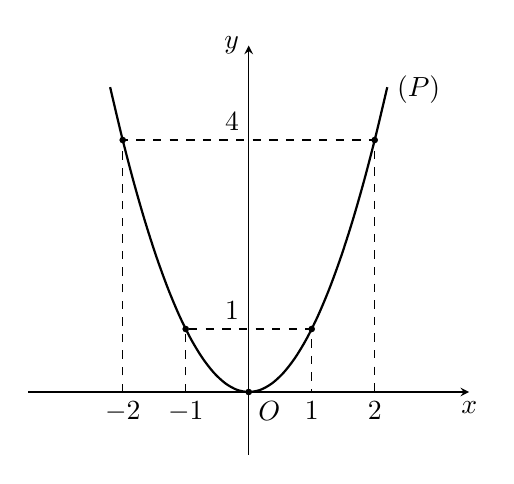
\begin{tikzpicture}[>=stealth, scale=0.8]
\draw[->] (-3.5,0) -- (3.5,0) node[below] {$x$};
\draw[->] (0,-1) -- (0,5.5) node[left] {$y$};
\fill (0,0) circle (1.5pt) node[below right] {$O$};
\draw[domain=-2.2:2.2, smooth, thick] plot (\x, {\x*\x});
\draw[dashed] (-2,0) node[below]{$-2$} |- (0,4) node[above left]{$4$} -| (2,0) node[below]{$2$};
\draw[dashed] (-1,0) node[below]{$-1$} |- (0,1) node[above left]{$1$} -| (1,0) node[below]{$1$};
\fill (-2,4) circle (1.5pt); \fill (2,4) circle (1.5pt);
\fill (-1,1) circle (1.5pt); \fill (1,1) circle (1.5pt);
\node[right] at (2.2, 4.8) {$(P)$};
\end{tikzpicture}
\end{center}
\textbf{b)} Tìm tọa độ giao điểm của $(P)$ và $(d)$ \hfill \textit{(0,5 điểm)} \par
Phương trình hoành độ giao điểm của $(P)$ và $(d)$ là:
$$ x^2 = -2x + 3 $$
$$ \Leftrightarrow x^2 + 2x - 3 = 0 $$
Vì $a + b + c = 1 + 2 + (-3) = 0$ nên phương trình có hai nghiệm:
$$ x_1 = 1; \quad x_2 = -3 $$
Với $x = 1 \Rightarrow y = (1)^2 = 1$. Ta được giao điểm thứ nhất là $(1; 1)$. \par
Với $x = -3 \Rightarrow y = (-3)^2 = 9$. Ta được giao điểm thứ hai là $(-3; 9)$. \par
Vậy tọa độ giao điểm của $(P)$ và $(d)$ là $(1; 1)$ và $(-3; 9)$.
}
\end{bt}

% nguồn: 2026-11-18_chuan_hoa_45_cau_ts10_vao_lop9 (nhập 18/11/2026)
\begin{bt}%[9D6H18-3]%[ma:02d569b7]
% nguon: Tuyển tập đề thi Tuyển sinh 10 TP.HCM
Cho parabol $(P): y = 2x^2$ và đường thẳng $(d): y = x + 3$.
\textbf{a)} Vẽ đồ thị $(P)$ trên hệ trục tọa độ. \par
\textbf{b)} Tìm tọa độ giao điểm của $(P)$ và $(d)$ bằng phép tính.
\loigiai{
\textbf{a)} Vẽ đồ thị $(P): y = 2x^2$ \hfill \textit{(1,0 điểm)} \par
Bảng giá trị:
\begin{center}
\begin{tabular}{|c|c|c|c|c|c|}
\hline
$x$ & $-2$ & $-1$ & $0$ & $1$ & $2$ \\
\hline
$y = 2x^2$ & $8$ & $2$ & $0$ & $2$ & $8$ \\
\hline
\end{tabular}
\end{center}
Đồ thị hàm số $(P)$ là một đường parabol đi qua gốc tọa độ $O$, nhận trục $Oy$ làm trục đối xứng và nằm phía trên trục hoành.
\begin{center}
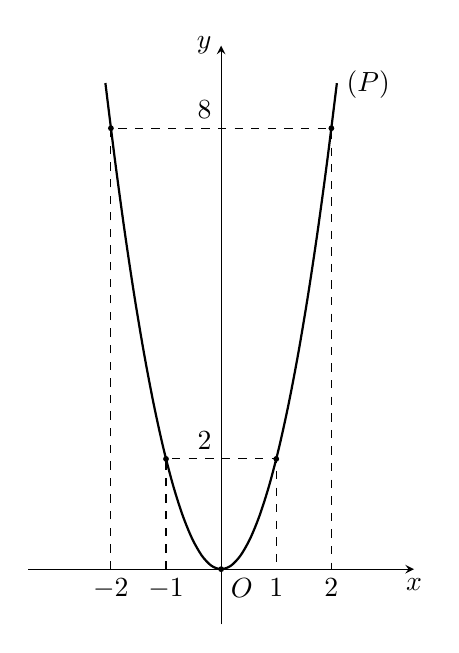
\begin{tikzpicture}[>=stealth, scale=0.7]
\draw[->] (-3.5,0) -- (3.5,0) node[below] {$x$};
\draw[->] (0,-1) -- (0,9.5) node[left] {$y$};
\fill (0,0) circle (1.5pt) node[below right] {$O$};
\draw[domain=-2.1:2.1, smooth, thick] plot (\x, {2*\x*\x});
\draw[dashed] (-2,0) node[below]{$-2$} |- (0,8) node[above left]{$8$} -| (2,0) node[below]{$2$};
\draw[dashed] (-1,0) node[below]{$-1$} |- (0,2) node[above left]{$2$} -| (1,0) node[below]{$1$};
\fill (-2,8) circle (1.5pt); \fill (2,8) circle (1.5pt);
\fill (-1,2) circle (1.5pt); \fill (1,2) circle (1.5pt);
\node[right] at (2.1, 8.8) {$(P)$};
\end{tikzpicture}
\end{center}
\textbf{b)} Tìm tọa độ giao điểm của $(P)$ và $(d)$ \hfill \textit{(0,5 điểm)} \par
Phương trình hoành độ giao điểm của $(P)$ và $(d)$ là:
$$ 2x^2 = x + 3 $$
$$ \Leftrightarrow 2x^2 - x - 3 = 0 $$
Vì $a - b + c = 2 - (-1) + (-3) = 0$ nên phương trình có hai nghiệm:
$$ x_1 = -1; \quad x_2 = \frac{3}{2} $$
Với $x = -1 \Rightarrow y = 2(-1)^2 = 2$. Ta được giao điểm thứ nhất là $(-1; 2)$. \par
Với $x = \frac{3}{2} \Rightarrow y = 2\left(\frac{3}{2}\right)^2 = \frac{9}{2}$. Ta được giao điểm thứ hai là $\left(\frac{3}{2}; \frac{9}{2}\right)$. \par
Vậy tọa độ giao điểm của $(P)$ và $(d)$ là $(-1; 2)$ và $\left(\frac{3}{2}; \frac{9}{2}\right)$.
}
\end{bt}

% nguồn: 2026-11-18_chuan_hoa_45_cau_ts10_vao_lop9 (nhập 18/11/2026)
\begin{bt}%[9D6H18-3]%[ma:2d79bb6c]
% nguon: Tuyển tập đề thi Tuyển sinh 10 TP.HCM
Cho parabol $(P): y = \frac{1}{4}x^2$.
\textbf{a)} Vẽ đồ thị $(P)$ trên mặt phẳng tọa độ. \par
\textbf{b)} Gọi $A$ và $B$ là hai điểm thuộc $(P)$ có hoành độ lần lượt là $-2$ và $4$. Tính diện tích tam giác $OAB$.
\loigiai{
\textbf{a)} Vẽ đồ thị $(P)$ \hfill \textit{(1,0 điểm)}\par
Bảng giá trị:
\begin{center}
\begin{tabular}{|c|c|c|c|c|c|}
\hline
$x$ & $-4$ & $-2$ & $0$ & $2$ & $4$ \\
\hline
$y = \frac{1}{4}x^2$ & $4$ & $1$ & $0$ & $1$ & $4$ \\
\hline
\end{tabular}
\end{center}
Đồ thị hàm số $(P)$ là đường parabol đi qua gốc tọa độ $O$, nhận trục $Oy$ làm trục đối xứng và nằm phía trên trục hoành.
\begin{center}
\begin{tikzpicture}[>=stealth, scale=0.8]
\draw[->] (-5,0) -- (5,0) node[below] {$x$};
\draw[->] (0,-1) -- (0,5) node[left] {$y$};
\fill (0,0) circle (1.5pt) node[below right] {$O$};
\draw[domain=-4.2:4.2, smooth, thick] plot (\x, {0.25*\x*\x});
\draw[dashed] (-4,0) node[below]{$-4$} |- (0,4) node[above left]{$4$} -| (4,0) node[below]{$4$};
\draw[dashed] (-2,0) node[below]{$-2$} |- (0,1) node[above left]{$1$} -| (2,0) node[below]{$2$};
\fill (-4,4) circle (1.5pt); \fill (4,4) circle (1.5pt);
\fill (-2,1) circle (1.5pt); \fill (2,1) circle (1.5pt);
\end{tikzpicture}
\end{center}
\textbf{b)} Tính diện tích tam giác $OAB$ \hfill \textit{(0,5 điểm)}\par
Với $x_A = -2 \Rightarrow y_A = \frac{1}{4}(-2)^2 = 1$. Ta có $A(-2; 1)$.\par
Với $x_B = 4 \Rightarrow y_B = \frac{1}{4}(4)^2 = 4$. Ta có $B(4; 4)$.\par
Gọi phương trình đường thẳng $AB$ là $y = ax + b$.
Thay tọa độ $A, B$ vào, ta có hệ:
$$ \heva{&-2a + b = 1 \\ &4a + b = 4} \Leftrightarrow \heva{&6a = 3 \\ &b = 1 + 2a} \Leftrightarrow \heva{&a = \frac{1}{2} \\ &b = 2} $$
Đường thẳng $AB$ có phương trình $y = \frac{1}{2}x + 2$. Gọi $C$ là giao điểm của $AB$ với trục $Oy$, ta có $C(0; 2) \Rightarrow OC = 2$.\par
Diện tích tam giác $OAB$ được chia thành hai tam giác vuông $OAC$ và $OBC$ chung cạnh đáy $OC$:
$$ S_{OAB} = S_{OAC} + S_{OBC} = \frac{1}{2} \cdot OC \cdot |x_A| + \frac{1}{2} \cdot OC \cdot |x_B| $$
$$ S_{OAB} = \frac{1}{2} \cdot 2 \cdot |-2| + \frac{1}{2} \cdot 2 \cdot |4| = 2 + 4 = 6 \text{ (đvdt).} $$
}
\end{bt}

% nguồn: 2026-11-18_chuan_hoa_45_cau_ts10_vao_lop9 (nhập 18/11/2026)
\begin{bt}%[9D6H18-3]%[ma:05be1f49]
% nguon: Tuyển tập đề thi Tuyển sinh 10 TP.HCM
Cho parabol $(P): y = -\frac{1}{2}x^2$.
\textbf{a)} Vẽ đồ thị $(P)$ trên hệ trục tọa độ. \par
\textbf{b)} Một cổng vòm có dạng parabol $(P)$ với đơn vị đo trên các trục là mét. Biết rằng mặt đường đi ngang qua vòm cầu ứng với đường thẳng $y = -2$. Tính bề rộng của mặt đường đi dưới cổng vòm đó.
\loigiai{
\textbf{a)} Vẽ đồ thị $(P)$ \hfill \textit{(1,0 điểm)}\par
Bảng giá trị:
\begin{center}
\begin{tabular}{|c|c|c|c|c|c|}
\hline
$x$ & $-4$ & $-2$ & $0$ & $2$ & $4$ \\
\hline
$y = -\frac{1}{2}x^2$ & $-8$ & $-2$ & $0$ & $-2$ & $-8$ \\
\hline
\end{tabular}
\end{center}
Đồ thị hàm số $(P)$ là đường parabol đi qua gốc tọa độ $O$, nhận trục $Oy$ làm trục đối xứng và nằm phía dưới trục hoành.
\begin{center}
\begin{tikzpicture}[>=stealth, scale=0.7]
\draw[->] (-5,0) -- (5,0) node[above] {$x$};
\draw[->] (0,-9) -- (0,1) node[right] {$y$};
\fill (0,0) circle (1.5pt) node[above right] {$O$};
\draw[domain=-4.2:4.2, smooth, thick] plot (\x, {-0.5*\x*\x});
\draw[dashed] (-4,0) node[above]{$-4$} |- (0,-8) node[below left]{$-8$} -| (4,0) node[above]{$4$};
\draw[dashed] (-2,0) node[above]{$-2$} |- (0,-2) node[below left]{$-2$} -| (2,0) node[above]{$2$};
\fill (-4,-8) circle (1.5pt); \fill (4,-8) circle (1.5pt);
\fill (-2,-2) circle (1.5pt); \fill (2,-2) circle (1.5pt);
\end{tikzpicture}
\end{center}
\textbf{b)} Tính bề rộng mặt đường \hfill \textit{(0,5 điểm)}\par
Mặt đường tương ứng với các điểm trên $(P)$ có tung độ $y = -2$. Ta xét phương trình:
$$ -\frac{1}{2}x^2 = -2 \Leftrightarrow x^2 = 4 \Leftrightarrow \heva{&x = 2 \\ &x = -2} $$
Do đó, cổng vòm chạm mặt đường tại hai điểm có tọa độ $(2; -2)$ và $(-2; -2)$.\par
Bề rộng của mặt đường đi dưới cổng vòm chính là khoảng cách giữa hai hoành độ này:
$$ \text{Bề rộng} = 2 - (-2) = 4 \text{ (m)} $$
Vậy bề rộng của mặt đường đi dưới cổng vòm là $4\text{ m}$.
}
\end{bt}

% nguồn: 2026-11-18_chuan_hoa_45_cau_ts10_vao_lop9 (nhập 18/11/2026)
\begin{bt}%[9D6H18-3]%[ma:0e41f170]
% nguon: Tuyển tập đề thi Tuyển sinh 10 TP.HCM
Cho hàm số $y = -2x^2$ có đồ thị là $(P)$.
\textbf{a)} Vẽ $(P)$ trên mặt phẳng tọa độ $Oxy$. \par
\textbf{b)} Đường thẳng $d: y = -8$ cắt đồ thị $(P)$ tại hai điểm phân biệt $M, N$. Tính chu vi tam giác $OMN$.
\loigiai{
\textbf{a)} Vẽ đồ thị $(P)$ \hfill \textit{(1,0 điểm)}\par
Bảng giá trị:
\begin{center}
\begin{tabular}{|c|c|c|c|c|c|}
\hline
$x$ & $-2$ & $-1$ & $0$ & $1$ & $2$ \\
\hline
$y = -2x^2$ & $-8$ & $-2$ & $0$ & $-2$ & $-8$ \\
\hline
\end{tabular}
\end{center}
Đồ thị hàm số $(P)$ là đường parabol đi qua gốc tọa độ $O$, nhận trục $Oy$ làm trục đối xứng và nằm phía dưới trục hoành.
\begin{center}
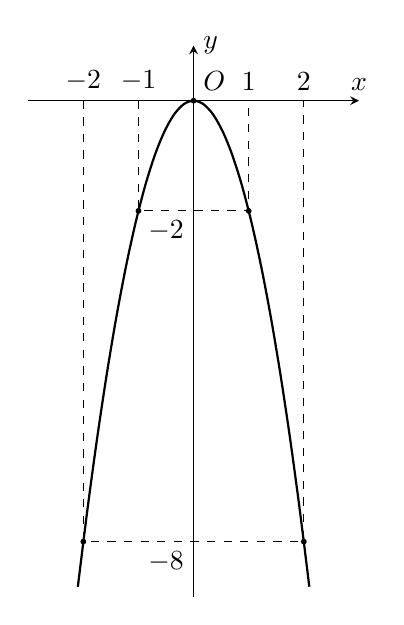
\begin{tikzpicture}[>=stealth, scale=0.7]
\draw[->] (-3,0) -- (3,0) node[above] {$x$};
\draw[->] (0,-9) -- (0,1) node[right] {$y$};
\fill (0,0) circle (1.5pt) node[above right] {$O$};
\draw[domain=-2.1:2.1, smooth, thick] plot (\x, {-2*\x*\x});
\draw[dashed] (-2,0) node[above]{$-2$} |- (0,-8) node[below left]{$-8$} -| (2,0) node[above]{$2$};
\draw[dashed] (-1,0) node[above]{$-1$} |- (0,-2) node[below left]{$-2$} -| (1,0) node[above]{$1$};
\fill (-2,-8) circle (1.5pt); \fill (2,-8) circle (1.5pt);
\fill (-1,-2) circle (1.5pt); \fill (1,-2) circle (1.5pt);
\end{tikzpicture}
\end{center}
\textbf{b)} Tính chu vi tam giác $OMN$ \hfill \textit{(0,5 điểm)}\par
Phương trình hoành độ giao điểm của $(P)$ và $d$:
$$ -2x^2 = -8 \Leftrightarrow x^2 = 4 \Leftrightarrow x = \pm 2 $$
Ta được tọa độ hai giao điểm là $M(-2; -8)$ và $N(2; -8)$.\par
Độ dài cạnh $MN = 2 - (-2) = 4$.\par
Áp dụng định lý Pythagore để tính $OM$ và $ON$ (với $OM = ON$ do tính đối xứng):
$$ OM = \sqrt{(-2)^2 + (-8)^2} = \sqrt{4 + 64} = \sqrt{68} = 2\sqrt{17} $$
Do đó $ON = 2\sqrt{17}$.\par
Chu vi tam giác $OMN$ là:
$$ P = OM + ON + MN = 2\sqrt{17} + 2\sqrt{17} + 4 = 4 + 4\sqrt{17} \text{ (đvđd).} $$
}
\end{bt}
